%=========================================================================
% (c) 2011, 2012 Josef Lusticky

\chapter{Hardware real-time support}
%! TODO
%TODO: Distinguish between TIME and CLOCK
%We need clock~\cite{timecounters}.
\begin{figure}
	\centering
	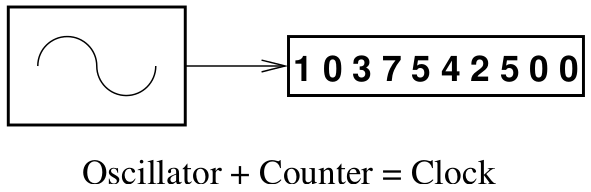
\includegraphics[width=6cm,keepaspectratio]{fig/clock.png}
	\caption{Clock by P. Kamp}
	\label{fig:hw-clock}
	%\bigskip
\end{figure}
For keeping, measuring and resolving time computer needs a clock.
Computer clock is an electronic device that counts oscillations in a
quartz crystal oscillator with a particular frequency~\cite{thesis-sync}.
These clocks are essentially timers associated with a counter register and
are capable of generating a hardware interrupt.
The counter register counts the oscillations of the crystal.
When the counter registers reaches a specific value,
an interrupt is generated.
Such interrupt is called a clock tick and at each clock tick,
interrupt service routine increments a system clock value stored in memory~\cite{thesis-sync}.

In a typical computer clock design, the clock oscillator drives a counter that produces processor interrupts at
fixed tick intervals in the range 1-20 ms.
At each tick interrupt a software clock variable is updated by the
number of microseconds or nanoseconds in the tick interval~\cite{timecounters}.


There are two different types of interrupts - hardware and software interrupts.

A typical desktop computer today includes CPU based on Intel x86 architecture.
Real-Time Clock (RTC) in CMOS memory that is battery powered

Unfortunately Intel x86 architecture is heavily influenced by backward compatibility,
and many hardware configurations are in use today -
e.g. the time value can also be stored in Binary Code Digit (BCD) encoding in RTC.

In year 19xx /, Starting with Intel 386,
Intel introduced
Programmable Interrupt Controller (PIT) Intel 8253 and 8254 - 3 counters (counter 0 interrupt to OS)

The problem with this device is that it only has
8bit bus-width, so reading a 16 bit timestamp takes
3 I/O operations: one to latch the count in an internal register,
and two to read the high and low parts
of that register respectively~\cite{timecounters}.
Obviously, on multi-CPU systems this cannot be
done without some kind of locking mechanism
preventing the other CPUs from trying to do the
same thing at the same time~\cite{timecounters}.


Used by historic versions of Linux
=> read initial time from RTC, setup PIT and interrupts (IRQ 0, INT 8), increment jiffies on every interrupt, provide application resolution of jiffies

init/main.c - time\_init() - read from RTC and save to startup\_time
kernel/sched.c - sched\_init() = PTI setup for interrupts - LATCH (1193180/HZ)
kernel/system\_call.s - timer\_interrupt() in assembly - increments jiffies

The current real time is provided by CURRENT\_TIME (startup\_time+jiffies/HZ) => since jiffies is integer and HZ is 100 => resolution of 10ms.
kernel/sys.c - sys\_time() - CURRENT\_TIME returned

\section{Clock quality}

\section{Interrupts}
Older x86 processors used an interrupt mechanism to switch from
user-space to kernel-space, but new x86 processors provide instructions
that optimize this transition (using sysenter and sysexit instructions)~\cite{ibm-linux-system-calls}.


TICK - http://www.ntp.org/ntpfaq/NTP-s-sw-clocks-tick.htm


- software:
The Kernel Discipline =  kernel clock model RFC 1589

However, some clock implementations do not allow small corrections to be applied to the system clock, and there is no standard interface to monitor the system clock's quality.
=> divide problem (in RFC)
